\documentclass[12pt]{article}
\usepackage[english,russian]{babel}
\usepackage[a4paper, margin=0.5cm, bottom=1.5cm]{geometry}
\usepackage{ragged2e} % Улучшенное выравнивание текста
\usepackage{graphicx} % Для добавления иллюстраций
\usepackage{tabularx} % Таблицы
\usepackage{icomma} % Делает запятую в формулах более "интеллектуальной"
\usepackage{lipsum} 
\usepackage{paracol} % Разбиение текста на колонки
\usepackage{amsmath} % Математические формулы
\usepackage{fancyhdr} % Настройка стиля страницы

\graphicspath{{./img/}} % Путь до картинок

\columnratio{0.25,0.75} % Соотношение размеров колонок
\setlength{\emergencystretch}{3em} % Максимальное расстояние между словами

\begin{document}
    % \documentclass[12pt]{article}
% \usepackage[english,russian]{babel}
% \usepackage[a4paper, margin=0.5cm, bottom=1.5cm]{geometry}
% \usepackage{fancyhdr} % Настройка стиля страницы

% \begin{document}
    \thispagestyle{fancy} % Стиль страницы с верхним и нижним колонтитулами
    \fancyhead{} % Очистить верхний колонтитул
    \fancyfoot{} % Очистить нижний колонтитул
    \fancyfoot[C]{Санкт-Петербург 2024}
    
    \begin{center}
        МИНИСТЕРСТВО НАУКИ И ВЫСШЕГО ОБРАЗОВАНИЯ РОССИЙСКОЙ ФЕДЕРАЦИИ

        \vspace{2em}

        ФЕДЕРАЛЬНОЕ ГОСУДАРСТВЕННОЕ АВТОНОМНОЕ ОБРАЗОВАТЕЛЬНОЕ УЧРЕЖДЕНИЕ ВЫСШЕГО ОБРАЗОВАНИЯ\\
        \large{«Национальный исследовательский университет ИТМО»}

        \vspace{2em}
        \Large{ФАКУЛЬТЕТ ПРОГРАММНОЙ ИНЖЕНЕРИИ И КОМПЬЮТЕРНОЙ ТЕХНИКИ}

        \vfill
        
        \textbf{\Large{Лабораторная работа № 6}}\\
        \vspace{1em}
        \Large{по дисциплине\\\vspace{1em}«ИНФОРМАТИКА»}\\
        \vspace{1em}
        \Large{Работа с системой компьютерной вёрстки \LaTeX}\\
        \vspace{1em}
        Вариант №\textbf{83}

        \vfill
    \end{center}

    \begin{flushright}
        \vfill
        \large{
            \textbf{\textit{Выполнил:}}\\
            Рязанов Никита Сергеевич\\
            студент группы P3107\\
            \vspace{1em}
            \textbf{\textit{Преподаватель:}}\\
            Балакшин Павел Валерьевич\\
            кандидат технических наук, доцент факультета ПИиКТ
        }
        \vfill
    \end{flushright}
    \clearpage
% \end{document}
    % \documentclass[12pt]{article}
% \usepackage[english,russian]{babel}
% \usepackage[a4paper, margin=0.5cm, bottom=1.5cm]{geometry}
% \usepackage{ragged2e} % Улучшенное выравнивание текста
% \usepackage{graphicx} % Для добавления иллюстраций
% \usepackage{tabularx} % Таблицы
% \usepackage{icomma} % Делает запятую в формулах более "интеллектуальной"
% \usepackage{lipsum} 
% \usepackage{paracol} % Разбиение текста на колонки
% \usepackage{amsmath} % Математические формулы
% \usepackage{fancyhdr} % Настройка стиля страницы

% \graphicspath{{./img/}} % Путь до картинок

% \columnratio{0.25,0.75} % Соотношение размеров колонок
% \setlength{\emergencystretch}{3em} % Максимальное расстояние между словами


% \begin{document}
    \pagestyle{fancy} % Стиль страницы с верхним и нижним колонтитулами
    \fancyhead{} % Очистить верхний колонтитул
    \fancyfoot{} % Очистить нижний колонтитул
    \pagenumbering{arabic} % Нумерация страниц арабскими цифрами
    \fancyfoot[L]{\textbf{\thepage}} % Номер страницы в левом части нижнего колонтитула
    \setcounter{page}{34} % Установить номер страницы
    \setcounter{figure}{4} % Установить номер картинки
    
    % Title

    \begin{paracol}{2}
        \begin{column}
        \end{column}
        
        \begin{column}
            \noindent\textbf{\LARGE{Решения задач}}\\
            \\
            \textbf{\large{М444, М445; Ф458-Ф461}}
        \end{column}
    \end{paracol} 

    % Article

    \begin{paracol}{2}
        \begin{column}
            \vspace*{\fill}
            \begin{figure}[h]
                \centering
                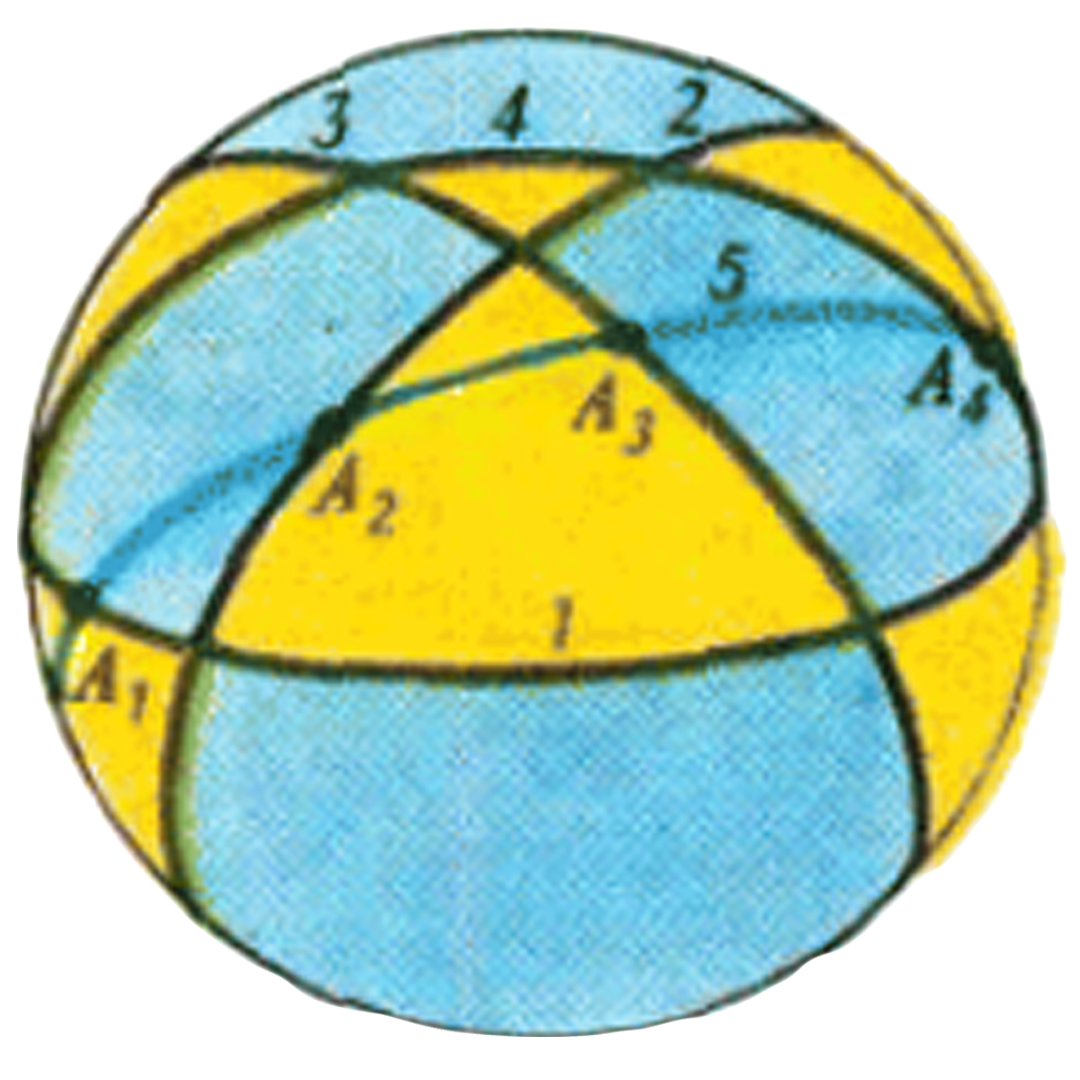
\includegraphics[width=0.8\linewidth]{sphere.png}
                \caption{Сфера}
                \label{fig:sphere}
            \end{figure}

            \begin{figure}[h]
                \centering
                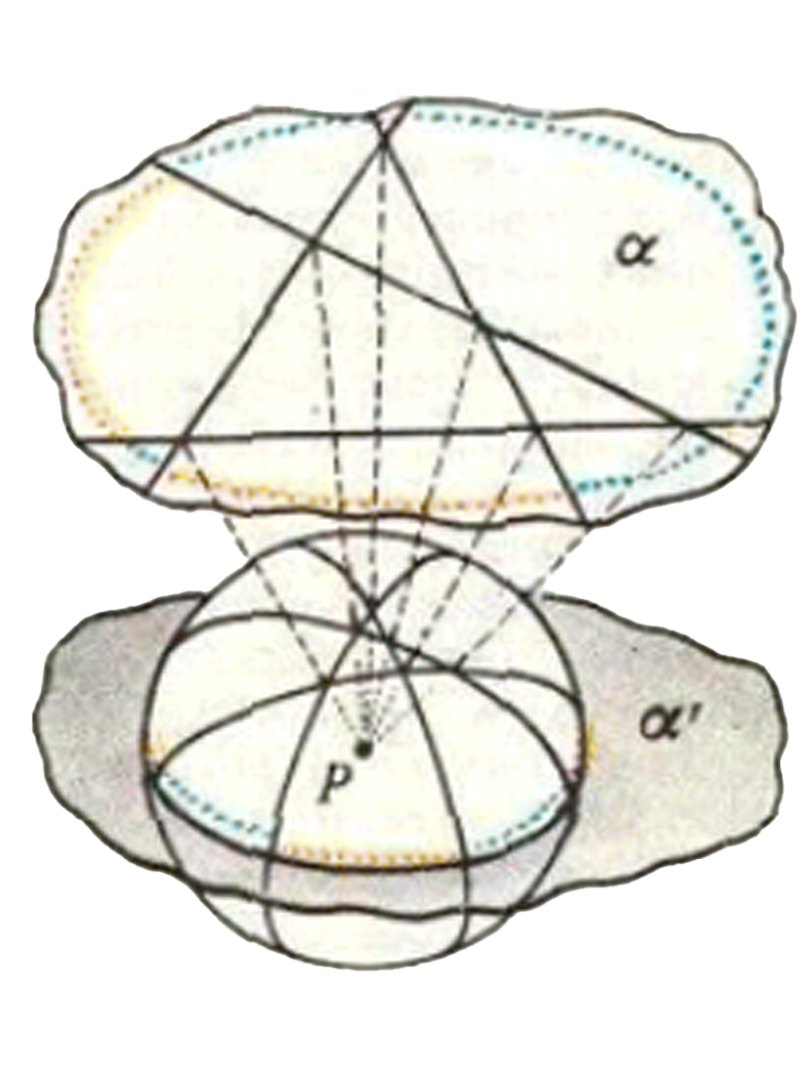
\includegraphics[width=0.8\linewidth]{sphere-with-plane.png}
                \caption{Сфера с плоскостью $\alpha$}
                \label{fig:sphere-with-plane}
            \end{figure}
            \vspace*{\fill}
        \end{column}

        \begin{column}
            \noindent Этот ответ у нас получился так:\\
            \\
            \begin{tabularx}{\linewidth}{
                |>{\hsize=1.8\hsize\linewidth=\hsize\raggedright\arraybackslash}X
                |>{\hsize=0.73\hsize\linewidth=\hsize\centering\arraybackslash}X 
                |>{\hsize=0.73\hsize\linewidth=\hsize\centering\arraybackslash}X 
                |>{\hsize=0.73\hsize\linewidth=\hsize\centering\arraybackslash}X | }
                \hline
                &5-угольников&4-угольников&3-угольников\\
                \hline
                4 круга разбивают сферу на&0&6&8\\
                \hline
                5-й круг оставляет нетронутыми&\vfill0&\vfill2&\vfill4\\
                разбивает 3-угольники на&0&2&4\\
                разбивает 4-угольники на&2&$4=2+2$&2\\
                \hline
                \rightline{Итого\ldots}&2&10&10\\
                \hline
            \end{tabularx}\\
            \\
            А теперь покажем. как этот же ответ получить намного проще.\\
            \so{Второе решение}. Спроектируем сферу из центра $P$ на плоскость $\alpha$, параллельную \textbf{экватору} $O$. Тогда пара симметричных $n$-угольников на сфере, не примыкающих к $O$, отобразится на $n$-угольник в плоскости $\alpha$, а пара $n$-угольников, примыкающих к $O$ --- на $(n-2)$ угол; пользуясь результатом задачи а) --- единственностью разбиения плоскости четырьмя прямыми и первой табличкой, --- мы заключаем, что любые пять больших кругов разбивают сферу на два пятиугольника (их проекция --- 3-угол), $2(1+4)=10$ четырехугольников (из них восемь примыкает к данному большому кругу O, и эти четыре пары проектируются на 2-углы), и $2(2+3)=10$ треугольников (из них шесть примыкают к большому кругу $O$). Те, кто знаком с понятием проективной плоскости (см. например. <<Квант>>. 1974. № 3), заметят, конечно, что «проекция», о которой мы говорим, более естественно объясняется как отображение сферы на \textit{проективную плоскость} (при этом отображении две диаметрально противоположные точки сферы склеиваются в одну, образы всех больших кругов --- прямые, в том числе образ круга \textit{O---бесконечно удаленная прямая}).\\
            Рисунок \ref{fig:sphere-with-plane}, иллюстрирующий второе решение, нужно пояснить. Поскольку «бесконечно удаленную прямую» нарисовать трудно, мы на рисунке 6 очень близко к большому кругу---экватору $O$ --- провели пунктиром параллель; ее образом при проекции будет окружность очень большого радиуса в плоскости $\alpha$, содержащая внутри себя все точки пересечения четырех прямых; эти прямые разбивают возникающий на плоскости «очень большой круг» на 11 областей: «пятиугольник», пять «треугольников» и пять «четырехугольников»; возвращаясь с плоскости на сферу, получаем после удвоения ответ.\\
            В заключение заметим, что во всех трех задачах не только вид частей разбиения (число сторон), но и их взаимное расположение определяются однозначно.\\
            Предлагаем читателям «Кванта» в качестве задачи для исследования выяснить, какие бывают разбиения сферы шестью большими кругами или плоскости --- пятью прямыми (здесь уже нет единственности). Самое трудное здесь, по-видимому, доказать то, что найдены все возможные варианты разбиения.\\
            \rightline{\textit{Н . Васильев}}
        \end{column}
    \end{paracol}
    
    \begin{paracol}{2}
        \begin{column}
        \end{column}

        \begin{column}
            \noindent\LARGE{$\diamond$}
            \vspace{0.5cm}
        \end{column}
    \end{paracol}
    
    \begin{paracol}{2}
        \begin{column}
            \noindent
            \textbf{М445}. \textit{Центры одинаковых непересекающихся окружностей находятся в центрах правильных шестиугольников, покрывающих плоскость так, как указано на рисунке 7. 
            Пусть $M$ --- многоугольник с вершинами в центрах окружностей. 
            Окрасим в красный цвет те окружности или части (дуги), которые лежат внутри $M$. 
            Покажите, что сумма градусных величин красных дуг равна $C \cdot 180^{\circ}$, где $C = C(M)$ --- целое число, и дайте этому числу геометрическую интерпретацию.}
        \end{column}
        

        \begin{column}
            \noindent
            Заметим. что центры правильных шестиугольников находятся в вершинах ромбов (сторона ромба --- удвоенная апофема шестиугольника, угол при вершине равен 60$^{\circ}$). 
            Таким образом, мы имеем \textit{ромбическую решетку} на плоскости; 
            вершины ромбов --- узлы решетки (см. рис. 7). 
            Далее, если многоугольник \textit{M} c вершинами в узлах представлен в виде объединения многоугольников $A_1, \ldots, A_k$ (с вершинами в узлах): $M = \bigcup\limits_{i=l}^{k} A_{i}$, то
            \[ C(M) = C(A_1)+\ldots+C(A_k);\] 
            про такую функцию говорят, что она \textit{аддитивна}. 
            Отсюда следует, что если многоугольник $M$ с вершинами в узлах представлен в виде объединения многоугольников $A_1, \ldots, A_k$, из которого удалено объединение многоугольников $B_1, \ldots, B_l$ ($A_i$ и $B_j$ --- с вершинами в узлах) --- см. рисунок 8; т. е. если 
            \begin{equation} \tag{*} M = \bigcup\limits_{i=1}^{k} A_i \setminus \bigcup\limits_{j=1}^{l} B_j  \text{, причем } \bigcup B_j \subset \bigcup A_i\end{equation} 
            (здесь $\times$ --- значок \textit{разности множеств} или \textit{дополнения}), то \[C(M)=\sum_{i=1}^{k} C(A_i) - \sum_{j=1}^{l} C(B_j).\]
        \end{column}
    \end{paracol}

% \end{document}
\end{document}
